% Analysis of the system
%
%
In this Section we will discusse the specifics of the system we propose as well as introduce our validated model of the system. With this model we were able to display the charging profile in Section \ref{sec:charging} and optimized for a charge to discharge ratio in section \ref{sec:chargedischarge}.

%---------- Design of the receiver
%
\begin{figure}[h!]
\centering
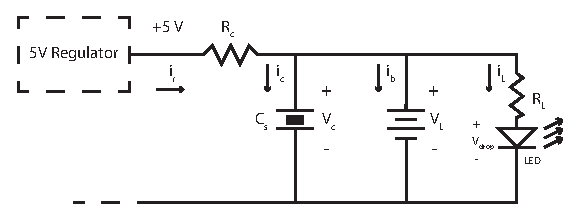
\includegraphics[width=0.8\textwidth]{rec_design.pdf}
\caption{Design of the Receiver of the wireless power transmitting system}
\label{fig:rec_des}
\end{figure}
%
Figure \ref{fig:rec_des} shows a low level schematic of the receiver and charging circuit which will be the main focus of our project. The induction current $i_r$ induced by the transmitter through magnetic coupling will be the main source of charging current. The current $i_c$ charges the super capacitor $C_s$ up to the capacity of $V_c$, in our case $V_c \leq 5$ Volts as this is the maximum voltage rating of our supercapacitor, $i_b$ charges the battery and $i_L$ is consumed by the current limiting resistor $R_L$  and a light source $LED$. Where $i_r = i_c + i_b +i_L$ . Now in analysis lets first consider the efficiency ${\eta}$ of the circuit. If $P_{o}$ is the power consumed by the receiver and $P_{i}$ is the power provided by the transmitter, ignoring small power drops across $D_r$ and $C_r$  then:
%
\begin{equation}\label{eq:effb}
 {\eta} = \frac{P_o}{P_i}
\end{equation}
%
where $P_o = V_{reg} \times i_r $ and $P_i = V_i \times i_s $. The receiving battery can provide $V_l = 3 $ Volts when fully charged. For a 3 Volts lithium-ion battery the output voltage normally drops by $0.2 $ Volts whenthe  battery is at $40 \%$ of its capacity and can go to $2.6 $ Volts when it is almost drained \cite{IAmp}. Therefor a slight dim in LED brightness can be observed as battery drains with time. To ensure a normal brightness of our \emph{LED} with a forward voltage drop of $V_{drop} = 1.7 $ Volts we choose need a current of $i_L = 20 $ mA. To determine the required resistance we used equation ~\ref{eq:load} and found $R_L = 65 \Omega $
%
\begin{equation}\label{eq:load}
 R_L = \frac{V_l - V_{drop}}{i_L}
\end{equation}
%
Using $P_L = {i_L}^2 \times R_L $ we can determine the power rating of $R_L$ that gives us $P_L = 400 \mu$ Watts. This is the power dissipated at $R_L$ and can be avoided if we use a LED that has exactly the same forward voltage drop $V_{drop}$ as the battery output $V_l$. This will remove the need for the resistor $R_L$. A LED is very sensitive to even small changes in the applied voltage. A voltage change of 0.1 Volt can cause the LED current $i_L$ to shoot up beyond the limits hence a more careful consideration is required if one chooses to omit the current limiting resistor $R_L$.
